\begin{figure}[ht]
    \vspace{.5cm}
    \centering
    \tikzstyle{block} = [rectangle, draw, text width=25em, inner sep=1ex, rounded corners, font=\small]
    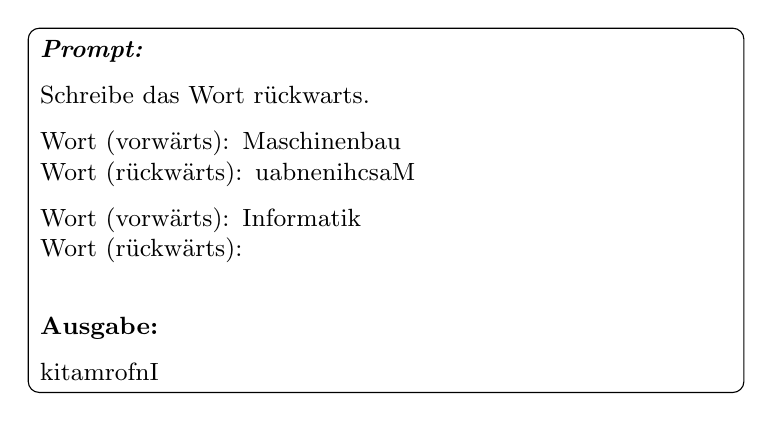
\begin{tikzpicture}
        \tikzset{node distance = 0.75cm and 1.5cm}
        % Main node with embedded tikzpicture
        \node (n1) at (0,0) [block] {
            \textbf{\textit{Prompt:}}\\[0.2cm]

            Schreibe das Wort rückwarts.\\[0.2cm]
            Wort (vorwärts): Maschinenbau\\
            Wort (rückwärts): uabnenihcsaM\\[0.2cm]
            Wort (vorwärts): Informatik\\
            Wort (rückwärts):\\[0.6cm]
            
            \textbf{Ausgabe:}\\[0.2cm]
            
            kitamrofnI};
    \end{tikzpicture}
    \caption{\textit{One-Shot Prompt} Beispiel}
    \label{fig:prompt-one}
\end{figure}
